\chapter{Prüfungsaufgaben}

In diesem Abschnitt werden einige Ideen für Prüfungsaufgaben vorgestellt, die das Verständnis der Lernenden für Netzwerkkonzepte und deren praktische Anwendung testen.

\begin{myexercise}[\textbf{Theoriefrage}: IP-Adresse vs. Port]

    \textbf{Aufgabe:} Erklären Sie den Unterschied zwischen einer IP-Adresse und einem Port. Warum sind beide notwendig, um eine Netzwerkverbindung herzustellen?
    \\[.5cm]
    \textbf{Bewertung (max. 5 Punkte):}
    \begin{itemize}
        \item Unterschied IP vs. Port klar beschrieben (2)
        \item Notwendigkeit beider für eindeutige Dienst-Adressierung (2)
        \item Präzise Fachsprache / Struktur (1)
    \end{itemize}
    \begin{myanswer}
        Eine IP-Adresse identifiziert ein Gerät in einem Netzwerk eindeutig, ähnlich wie eine Hausadresse in der realen Welt. Sie gibt an, wohin Datenpakete gesendet werden sollen. Ein Port hingegen ist eine nummerische Kennung, die auf einem Gerät verwendet wird, um verschiedene Dienste oder Anwendungen zu unterscheiden. Während die IP-Adresse das Zielgerät angibt, spezifiziert der Port den spezifischen Dienst (z.B. Webserver, E-Mail-Server) auf diesem Gerät. Beide sind notwendig, um sicherzustellen, dass Daten korrekt zugestellt werden.
    \end{myanswer}
\end{myexercise}

\begin{myexercise}[\textbf{Debugging-Aufgabe}: Netzwerkfehler beheben]

    \textbf{Aufgabe:} Sie versuchen, Ihren \texttt{client.py} mit dem Server zu verbinden, erhalten aber die Fehlermeldung \texttt{ConnectionRefusedError}. Nennen Sie mindestens drei mögliche Ursachen für diesen Fehler und beschreiben Sie jeweils eine Lösungsmöglichkeit.
    \\[.5cm]
    \textbf{Bewertung (max. 9 Punkte):}
    \begin{itemize}
        \item Drei korrekte Ursachen (je 1) (3)
        \item Passende Lösungen zu jeder Ursache (je 1) (3)
        \item Klarheit / Prägnanz der Fehleranalyse (3)
    \end{itemize}
    \begin{myanswer}
        \begin{itemize}
            \item \textbf{Server läuft nicht:} Der Server wurde nicht gestartet oder ist abgestürzt. \textit{Lösung:} Starten Sie den Server und versuchen Sie die Verbindung erneut.
            \item \textbf{Falsche IP-Adresse oder Port:} Der Client versucht, sich mit einer falschen Adresse oder einem falschen Port zu verbinden. \textit{Lösung:} Überprüfen Sie die IP-Adresse und den Port im Code und passen Sie sie ggf. an.
            \item \textbf{Firewall blockiert die Verbindung:} Die Firewall auf dem Server- oder Client-Rechner blockiert den Netzwerkverkehr. \textit{Lösung:} Passen Sie die Firewall-Einstellungen an, um Verbindungen auf dem verwendeten Port zuzulassen.
        \end{itemize}
    \end{myanswer}
\end{myexercise}

% Define a simple macro for blanks (works in article)
\newcommand{\blank}[1]{\underline{\hspace{2cm}}}

\begin{myexercise}[\textbf{Lückentext}: Netzwerk-Grundlagen]

    In einem Computernetzwerk werden verschiedene Geräte miteinander verbunden, um Daten auszutauschen. Ein zentrales Element hierbei ist der \blank{Router}, welcher den Datenverkehr zwischen verschiedenen Netzwerken steuert. Innerhalb eines Netzwerks übernimmt ein \blank{Switch} die Verteilung der Datenpakete an die richtigen Geräte.

    Jedes Gerät in einem Netzwerk hat eine eindeutige \blank{IP}-Adresse. Dabei unterscheiden wir zwischen zwei Arten von Adressen: Während \blank{IPv4}-Adressen aus 32 Bit bestehen, nutzen \blank{IPv6}-Adressen 128 Bit und bieten dadurch eine wesentlich grössere Anzahl möglicher Adressen.

    Zur Verwaltung der Routen, die Datenpakete nehmen sollen, verwendet ein Router eine \blank{Routing-Tabelle}. Damit der Router weiss, wie gross ein Teilnetz ist, wird eine \blank{Subnetzmaske} verwendet. Diese Maske hilft dabei, die Netzwerk- und die Hostanteile einer IP-Adresse zu trennen.

    Um den Domain-Namen in eine IP-Adresse zu übersetzen, wird das \blank{DNS}-Protokoll verwendet. Möchte man die IP-Adresse eines Domain-Namens herausfinden, kann man den Befehl \blank{nslookup} nutzen.

    Für Diagnosezwecke gibt es verschiedene Befehle. Mit \blank{ping} kann man überprüfen, ob ein anderes Gerät im Netzwerk erreichbar ist. Um die Netzwerkkonfiguration eines Geräts anzuzeigen, verwendet man den Befehl \blank{ipconfig} (Windows) bzw. \blank{ifconfig} (Linux/macOS).

    Um eine zuverlässige Datenübertragung zu gewährleisten, wird das \blank{TCP}-Protokoll verwendet. Für den Abruf von Webseiten kommt das \blank{HTTP}-Protokoll zum Einsatz.
    \\[.5cm]
    \\[.5cm]
    \textbf{Bewertung (max. 13 Punkte):} Jede korrekt ausgefüllte Lücke (1 Punkt).
    \begin{myanswer}
        In einem Computernetzwerk werden verschiedene Geräte miteinander verbunden, um Daten auszutauschen. Ein zentrales Element hierbei ist der \textbf{Router}, welcher den Datenverkehr zwischen verschiedenen Netzwerken steuert. Innerhalb eines Netzwerks übernimmt ein \textbf{Switch} die Verteilung der Datenpakete an die richtigen Geräte.

        Jedes Gerät in einem Netzwerk hat eine eindeutige \textbf{IP}-Adresse. Dabei unterscheiden wir zwischen zwei Arten von Adressen: Während \textbf{IPv4}-Adressen aus 32 Bit bestehen, nutzen \textbf{IPv6}-Adressen 128 Bit und bieten dadurch eine wesentlich grössere Anzahl möglicher Adressen.

        Zur Verwaltung der Routen, die Datenpakete nehmen sollen, verwendet ein Router eine \textbf{Routing-Tabelle}. Damit der Router weiss, wie gross ein Teilnetz ist, wird eine \textbf{Subnetzmaske} verwendet. Diese Maske hilft dabei, die Netzwerk- und die Hostanteile einer IP-Adresse zu trennen.

        Um den Domain-Namen in eine IP-Adresse zu übersetzen, wird das \textbf{DNS}-Protokoll verwendet. Möchte man die IP-Adresse eines Domain-Namens herausfinden, kann man den Befehl \textbf{nslookup} nutzen.

        Für Diagnosezwecke gibt es verschiedene Befehle. Mit \textbf{ping} kann man überprüfen, ob ein anderes Gerät im Netzwerk erreichbar ist. Um die Netzwerkkonfiguration eines Geräts anzuzeigen, verwendet man den Befehl \textbf{ipconfig} (Windows) bzw. \textbf{ifconfig} (Linux/macOS).

        Um eine zuverlässige Datenübertragung zu gewährleisten, wird das \textbf{TCP}-Protokoll verwendet. Für den Abruf von Webseiten kommt das \textbf{HTTP}-Protokoll zum Einsatz.
    \end{myanswer}
\end{myexercise}

\begin{myexercise}[\textbf{Zuordnungsaufgabe}: Netzwerk-Schichten]

    Ordnen Sie die folgenden Erklärungen der richtigen Netzwerk-Schicht zu (Anwendungsschicht, Physikalische Schicht, Vermittlungsschicht, Transportschicht):
    \\[.5cm]
    \\[.5cm]
    \textbf{Bewertung (max. 8 Punkte):} Jede richtige Zuordnung (2 Punkte).

    \begin{enumerate}
        \item \textbf{Stellt die elektrische, mechanische und funktionale Verbindung zwischen Geräten her.}
        \item \textbf{Sorgt für die korrekte Übertragung von Datenpaketen zwischen Sender und Empfänger, inklusive Fehlererkennung und -behebung.}
        \item \textbf{Regelt die Weiterleitung von Datenpaketen zwischen verschiedenen Netzwerken und bestimmt den besten Weg zum Ziel.}
        \item \textbf{Stellt Dienste wie E-Mail, Webseiten oder Dateiübertragung für den Nutzer bereit.}
    \end{enumerate}

    \begin{myanswer}
        \begin{itemize}
            \item \textbf{Physikalische Schicht}: Stellt die elektrische, mechanische und funktionale Verbindung zwischen Geräten her.
            \item \textbf{Transportschicht}: Sorgt für die korrekte Übertragung von Datenpaketen zwischen Sender und Empfänger, inklusive Fehlererkennung und -behebung.
            \item \textbf{Vermittlungsschicht}: Regelt die Weiterleitung von Datenpaketen zwischen verschiedenen Netzwerken und bestimmt den besten Weg zum Ziel.
            \item \textbf{Anwendungsschicht}: Stellt Dienste wie E-Mail, Webseiten oder Dateiübertragung für den Nutzer bereit.
        \end{itemize}
    \end{myanswer}
\end{myexercise}

\begin{myexercise}[\textbf{Anwendungsaufgabe}: Netzwerkbefehle praktisch nutzen]

    Sie möchten herausfinden, ob Ihr Computer eine Verbindung zu einem Server im Internet herstellen kann. Beschreiben Sie, wie Sie mit den Befehlen \texttt{ping} und \texttt{nslookup} vorgehen würden und was die jeweilige Ausgabe bedeutet.
    \\[.5cm]
    \textbf{Bewertung (max. 6 Punkte):}
    \begin{itemize}
        \item Ablauf und Zweck von \texttt{ping} korrekt (3)
        \item Ablauf und Zweck von \texttt{nslookup} korrekt (3)
    \end{itemize}

    \begin{myanswer}
        Mit \texttt{ping} kann ich prüfen, ob der Server erreichbar ist, indem ich z.B. \texttt{ping google.com} eingebe. Die Ausgabe zeigt, ob Pakete erfolgreich gesendet und empfangen wurden. Mit \texttt{nslookup google.com} kann ich die IP-Adresse des Servers herausfinden. Die Ausgabe zeigt die zugehörige IP-Adresse und ggf. weitere DNS-Informationen.
    \end{myanswer}
\end{myexercise}

\begin{myexercise}[\textbf{Konzepte}: Client-Server-Architektur]

    Erklären Sie in eigenen Worten, wie die Client-Server-Architektur funktioniert und nennen Sie ein Beispiel aus dem Alltag, bei dem dieses Prinzip genutzt wird.
    \\[.5cm]
    \textbf{Bewertung (max. 5 Punkte):}
    \begin{itemize}
        \item Prinzip korrekt und strukturiert erklärt (3)
        \item Passendes Alltagsbeispiel (2)
    \end{itemize}

    \begin{myanswer}
        Bei der Client-Server-Architektur fordert ein Client (z.B. ein Browser) einen Dienst oder eine Ressource von einem Server an (z.B. eine Webseite). Der Server verarbeitet die Anfrage und schickt die Antwort zurück. Ein Beispiel ist das Abrufen einer Webseite: Der Browser ist der Client, der Webserver liefert die Seite.
    \end{myanswer}
\end{myexercise}

\begin{myexercise}[\textbf{Fehleranalyse}: Firewall und Netzwerkkommunikation]

    Sie haben ein Socket-Programm geschrieben, aber die Verbindung zwischen zwei Rechnern im lokalen Netzwerk funktioniert nicht. Nennen Sie zwei Möglichkeiten, wie eine Firewall die Kommunikation verhindern kann, und wie Sie das Problem lösen können.
    \\[.5cm]
    \textbf{Bewertung (max. 4 Punkte):}
    \begin{itemize}
        \item Zwei korrekte Firewall-Hindernisse (je 1) (2)
        \item Zwei passende Lösungsansätze (je 1) (2)
    \end{itemize}

    \begin{myanswer}
        Die Firewall kann entweder den verwendeten Port blockieren oder den gesamten eingehenden Netzwerkverkehr sperren. Lösung: Den Port in der Firewall freigeben oder eine Ausnahme für das Programm hinzufügen.
    \end{myanswer}
\end{myexercise}

\begin{myexercise}[\textbf{Programmieraufgabe}: Erweiterung eines Chat-Clients]\label{ex:erweiterungClient}

    Ihr Chat-Client kann bisher nur Nachrichten an einen Server senden und empfangen. Beschreiben Sie, wie Sie das Programm erweitern würden, damit mehrere Clients gleichzeitig Nachrichten austauschen können.
    \\[.5cm]
    \textbf{Bewertung (max. 12 Punkte):}
    \begin{itemize}
        \item Mehrfachverbindungen (Threading / Async / Select) Konzept (4)
        \item Verwaltung der Client-Sitzungen / Namensregistrierung (3)
        \item Mechanismus zum Weiterleiten / Broadcast / gezielte Zustellung (3)
        \item Sicherheit / Fehlerbehandlung / Ressourcenhinweis (Bonus bis +2)
    \end{itemize}

    \begin{myanswer}
        Der Server muss mehrere Verbindungen gleichzeitig verwalten, z.B. mit Threads. Jeder Client sendet seinen Namen beim Verbinden. Der Server leitet Nachrichten an den gewünschten Empfänger weiter, indem er die Namen und Verbindungen speichert und die Nachricht gezielt zustellt.
    \end{myanswer}
\end{myexercise}
\newpage
\begin{myexercise}[Projekt: Debugging und Erweiterung eines Chat-Clients]
    Ihr Entwicklerteam hat durch eine externe Agentur einen einfachen Chat-Client erstellen lassen, welcher jedoch einige Probleme aufweist. Die Verbindung zum Server bricht häufig ab, und es gibt keine Möglichkeit, Nachrichten an spezifische Nutzer zu senden. 

    Im Folgenden Projekt werden Sie als Gruppe diese Probleme analysieren und Lösungen implementieren. Zudem werden Sie einige Zusatzfunktionen hinzufügen, welche Ihre Agentur aus Kostengründen nicht realisieren konnte.

    \textbf{Aufgabenstellung:}
    \begin{enumerate}
        \item Analysieren Sie den bestehenden Code und identifizieren Sie die Ursachen für die Verbindungsabbrüche. Dokumentieren Sie Ihre Erkenntnisse.
        \item Erweitern Sie Ihren Chat-Client, indem Sie die Funktionalitäten aus \cref{ex:erweiterungClient} umsetzen.
    \end{enumerate} 

    \textbf{Bewertung (max. 20 Punkte):}
    \begin{itemize}
        \item Fehleranalyse und Dokumentation (8)
        \item Implementierung der Mehrfachverbindungen (Threading) (3)
        \item Verwaltung der Client-Sitzungen / Namensregistrierung (1.5 Punkte pro Aspekt, 3 total)
        \item Mechanismus zum Weiterleiten / Broadcast / gezielte Zustellung (1 Punkt pro Aspekt, 3 total)
        \item Sicherheit / Fehlerbehandlung / Ressourcenhinweis (1 Punkt pro Aspekt, 3 total)
    \end{itemize}

    Weitere 4 Punkte werden für den Arbeitsprozess und die Zusammenarbeit in der Gruppe vergeben. Halten Sie in einer separaten Dokumentation folgendes fest:
    \begin{itemize}
        \item Rollenverteilung und Aufgabenverteilung innerhalb der Gruppe.
        \item Kommunikationswege und Entscheidungsprozesse.
        \item Reflexion über die Zusammenarbeit und mögliche Verbesserungen.
    \end{itemize}

    Im Rahmen einer Mündlich-Prüfung werden Sie Ihre Lösungen präsentieren und die getroffenen Entscheidungen erläutern.

    Ihre Endnote wird wie folgt berechnet:
    \[\text{Endnote} = \Bigg(\left(\frac{\text{Projekt-Punkte}}{20}\right) \times \left(\frac{\text{Verständnis-Prozentzahl}}{100}\right)\Bigg)*5+1\]
\end{myexercise}


\begin{myexercise}[Wireshark-Netzwerkanalyse]

    Beschreiben Sie, welche Protokolle auf folgendem Screenshot von Wireshark zu sehen sind, währenddem Sie eine Webseite im Browser aufgerufen haben. Erklären Sie kurz die Rolle jedes Protokolls im Kommunikationsprozess.
    \\[.5cm]
    \textbf{Bewertung (max. 10 Punkte):}
    \begin{itemize}
        \item DNS-Anfrage und -Antwort (2)
        \item \gls{TCP}-Verbindungsaufbau mit 3-Wege-Handshake (2)
        %\item TLS Handshake + Verschlüsselungszweck (3)
        \item HTTP/HTTPS Rolle Request/Response (3)
    \end{itemize}

    \begin{figure}[H]
        \centering
        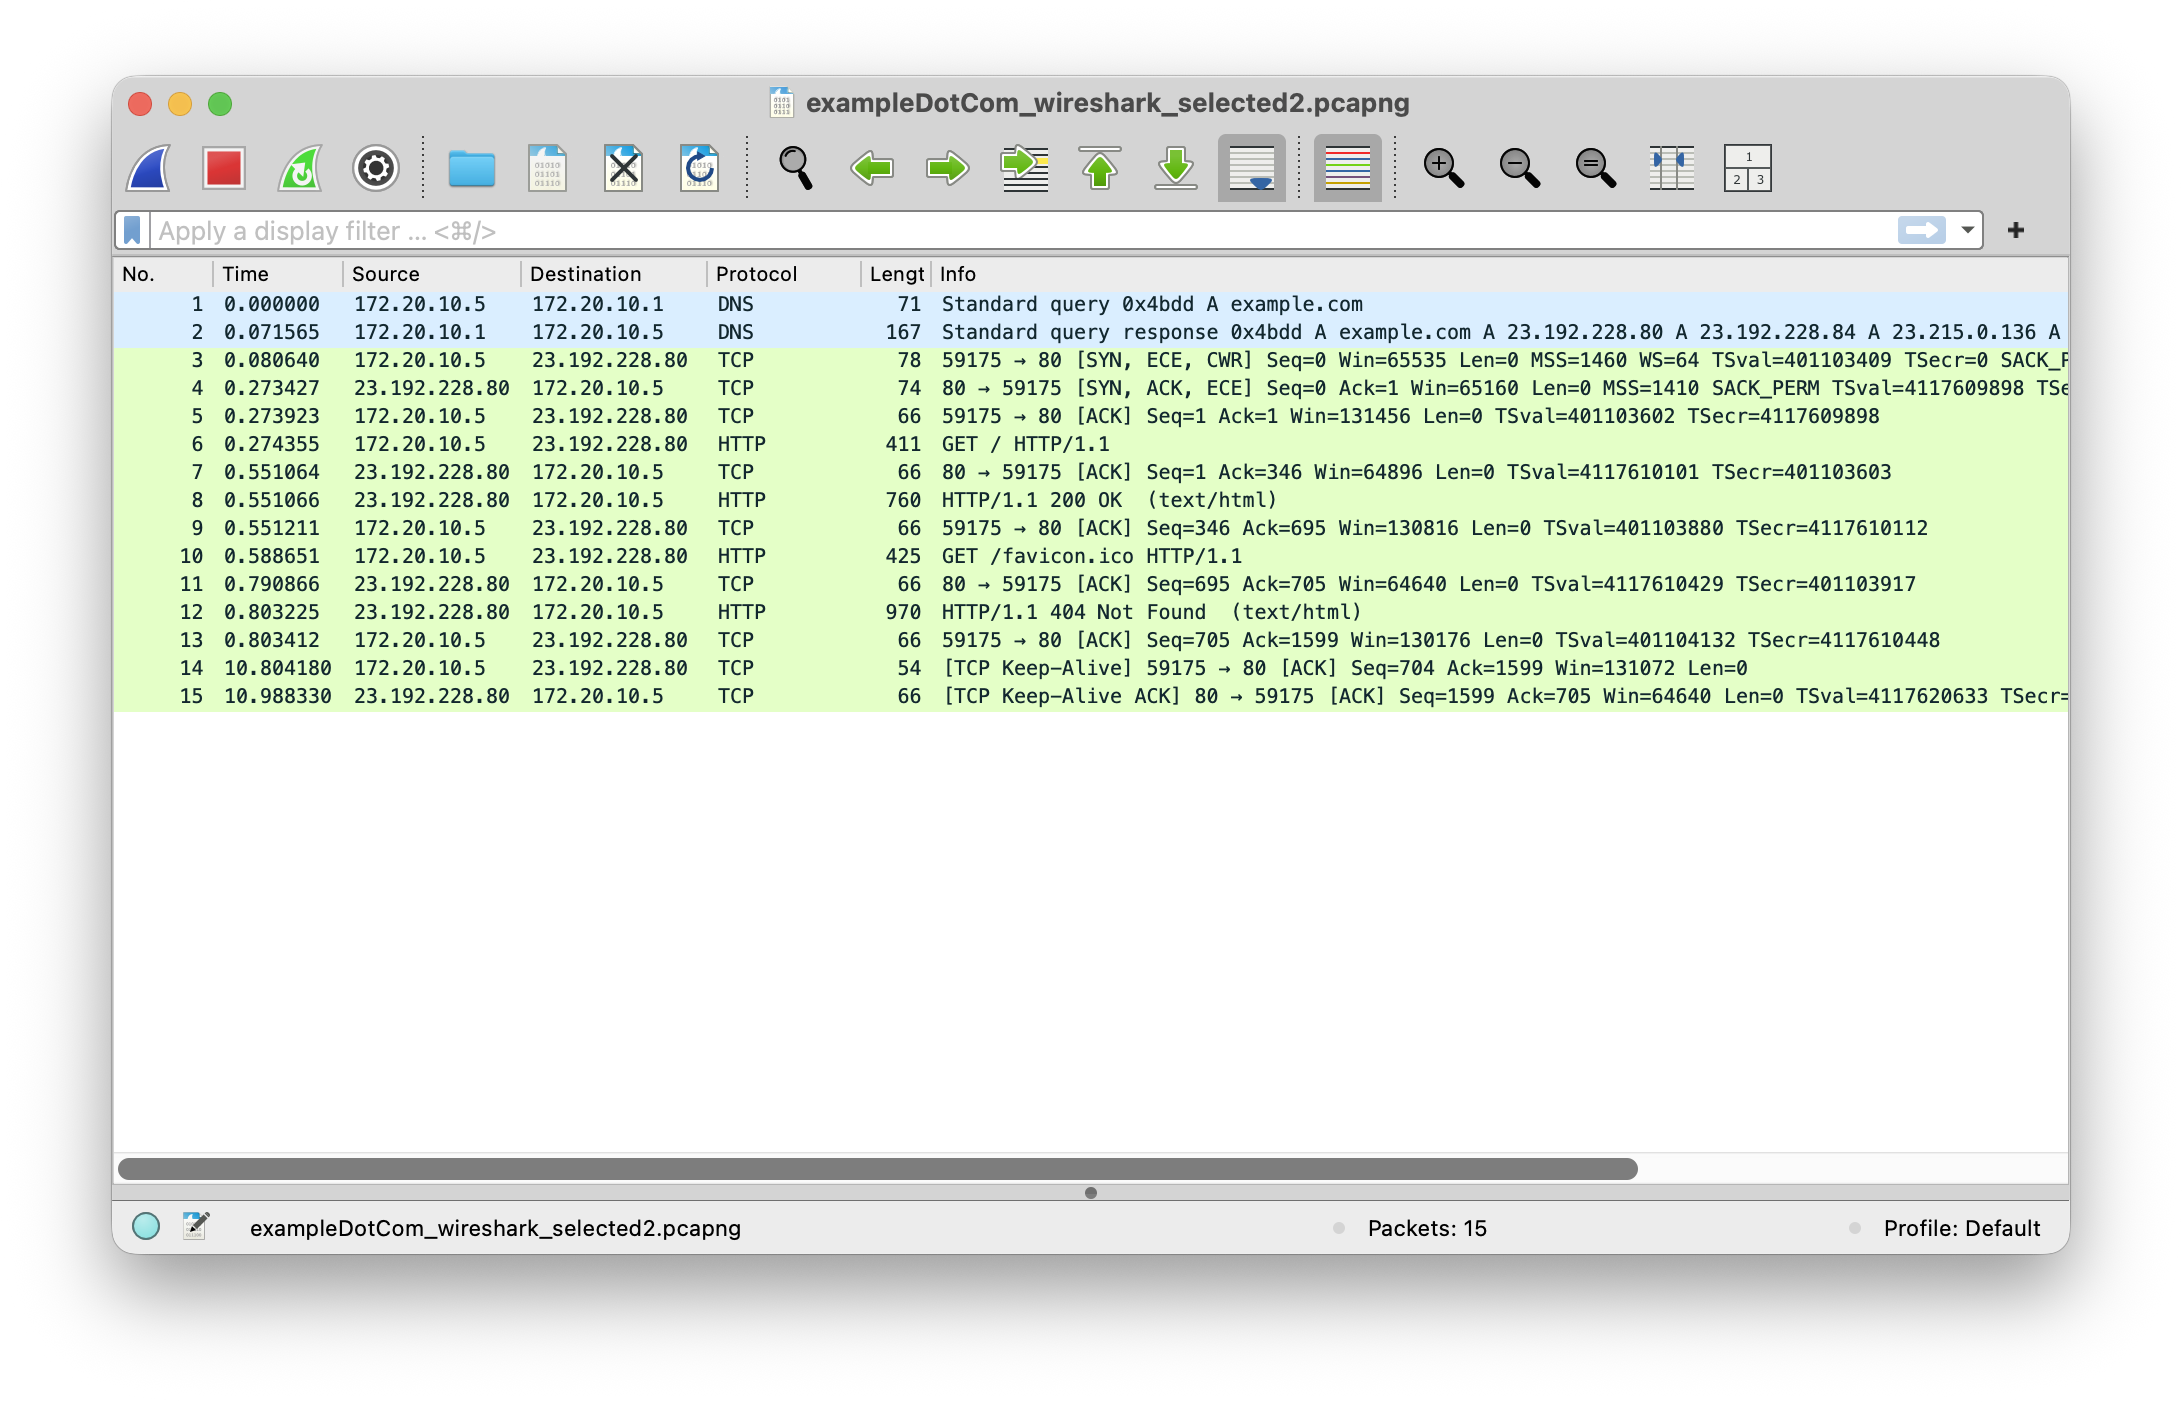
\includegraphics[width=\textwidth]{Grundlagen_Info/07_Netzwerke/Figures/exampleComWireshark}
        \caption{Wireshark-Screenshot während eines Webseitenaufrufs}
    \end{figure}

    \begin{myanswer}
        Auf dem Screenshot sind folgende Protokolle zu sehen:
        \begin{itemize}
            \item \textbf{\gls{DNS}:} Löst den Domainnamen in eine \gls{IP}-Adresse auf; erster Schritt beim Laden einer Webseite.
            \item \textbf{\gls{TCP}:} Baut eine zuverlässige Verbindung zwischen Client und Server auf (\texttt{SYN, SYN/ACK, ACK}) und transportiert die Daten.
            %\item \textbf{TLS:} Verschlüsselt die Kommunikation zwischen Browser und Server; Handshake legt Schlüssel fest.
            \item \textbf{HTTPS/HTTP:} Überträgt die eigentlichen Webinhalte (\texttt{GET}-/ \texttt{POST}-Requests / Responses), wäre bei HTTPS vollständig verschlüsselt und häufig unsichtbar.
        \end{itemize}
    \end{myanswer}
\end{myexercise}


\begin{myexercise}[\textbf{Reflexionsfrage}: Datenschutz und zentraler Server]
Beim Einsatz eines zentralen Relay-Servers für Chat-Kommunikation: Welche datenschutzrelevanten Risiken entstehen (Meta-Daten, Inhaltszugriff, Ausfallszenarien, Machtkonzentration)? Welche Alternativen zu zentralen Architekturen (z.B. Föderation, Peer-to-Peer, Ende-zu-Ende-Verschlüsselung) fördern digitale Souveränität? Formulieren Sie drei Gedanken dazu.
    \\[.5cm]
    \textbf{Bewertung (max. 6 Punkte):}
    \begin{itemize}
        \item Benennung zentraler Datenschutzrisiken (2)
        \item Analyse der Implikationen / Macht / Verfügbarkeit (2)
        \item Konkrete Alternativen zur Förderung von Souveränität (2)
    \end{itemize}
\begin{myanswer}
\begin{itemize}
    \item Zentraler Server bündelt Meta-Daten (wer kommuniziert wann mit wem) und kann Inhalte einsehen ohne Ende-zu-Ende-Verschlüsselung.
    \item Machtkonzentration schafft Abhängigkeit (Verfügbarkeit, Regeln, mögliche Zensur); Ausfall legt gesamte Kommunikation lahm.
    \item Föderierte oder Peer-to-Peer-Modelle verteilen Kontrolle; starke Ende-zu-Ende-Verschlüsselung mindert Einsicht; Transparenz und offene Protokolle fördern Souveränität.
\end{itemize}
\end{myanswer}
\end{myexercise}

\begin{myexercise}[\textbf{Diskussionsimpuls}: Datenminimierung]
Welche konkreten Massnahmen könnten in Ihrem Chat-Design umgesetzt werden, um Datenminimierung und Privatsphäre zu stärken (Speicherdauer, Verschlüsselung, Logging-Strategie)? Formulieren Sie drei kurze Vorschläge.
    \\[.5cm]
    \textbf{Bewertung (max. 6 Punkte):} Drei konkrete Massnahmen (je 2 Punkte) mit erkennbarem Bezug zu Privatsphäre / Minimierung.
\begin{myanswer}
\begin{itemize}
    \item Keine dauerhafte Speicherung von Nachrichten; flüchtiger Speicher im RAM.
    \item Ende-zu-Ende-Verschlüsselung mit kurzlebigen Schlüsseln (Forward Secrecy).
    \item Minimal-Logging: Nur technisch notwendige temporäre Session-IDs, keine persistente Nutzer-Historie.
\end{itemize}
\end{myanswer}
\end{myexercise}

\begin{myexercise}[\textbf{Theoriefrage}: NAT und Port-Forwarding]

    Erklären Sie, warum NAT (Network Address Translation) und Port-Forwarding notwendig sind, um eine Verbindung zu einem Server im Internet herzustellen, der sich hinter einem Router befindet.
    \\[.5cm]
    \textbf{Bewertung (max. 6 Punkte):}
    \begin{itemize}
        \item NAT-Funktionsprinzip korrekt erklärt (3)
        \item Rolle des Port-Forwarding für Erreichbarkeit (3)
    \end{itemize}

    \begin{myanswer}
        NAT übersetzt private IP-Adressen im lokalen Netzwerk in die öffentliche IP-Adresse des Routers. Damit ein Server im lokalen Netzwerk von aussen erreichbar ist, muss der Router eingehende Verbindungen über Port-Forwarding an die richtige lokale IP und den richtigen Port weiterleiten.
    \end{myanswer}
\end{myexercise}